\documentclass{beamer}

\usepackage[french]{babel}
\usepackage[T1]{fontenc}
\usepackage[utf8]{inputenc}

\usetheme{Warsaw}
\useoutertheme{infolines}

\usepackage{amsmath}
\usepackage{amssymb}
\usepackage{amsthm}
\usepackage{stmaryrd}

\usepackage{listings}
\usepackage{color}

\definecolor{mygreen}{rgb}{0,0.6,0}
\definecolor{mygray}{rgb}{0.5,0.5,0.5}
\definecolor{mymauve}{rgb}{0.58,0,0.82}

\lstset{ %
  backgroundcolor=\color{white},   % choose the background color
  basicstyle=\footnotesize,        % size of fonts used for the code
  breaklines=true,                 % automatic line breaking only at whitespace
  captionpos=b,                    % sets the caption-position to bottom
  commentstyle=\color{mygreen},    % comment style
  escapeinside={\%*}{*)},          % if you want to add LaTeX within your code
  keywordstyle=\color{blue},       % keyword style
  stringstyle=\color{mymauve},     % string literal style
}

\lstset{language=java} 

\usepackage[all]{xy}

%Les sous listes on des triangles
\setbeamertemplate{itemize item}[circle]
\setbeamertemplate{itemize subitem}[triangle]
%Les elements caché sont grisé
\beamertemplatetransparentcovered

\begin{document}

\title{Android - Les fondamentaux}
\author{Jérémy S. Cochoy}
\institute{INRIA Paris-Saclay | jeremy.cochoy@u-psud.fr}
\date{Novembre 2015}


\begin{frame}
\titlepage
\end{frame}

\begin{frame}
\tableofcontents
\end{frame}

\begin{frame}
\frametitle{La documentation}

\begin{block}{Votre nouveau livre de chevet.}
\begin{center}
\emph{https://developer.android.com/guide/index.html}
\end{center}
\end{block}

\end{frame}

\section{Appareille Photo - Correction}

\begin{frame}
\frametitle{TP Appareille Photo}
\begin{center}
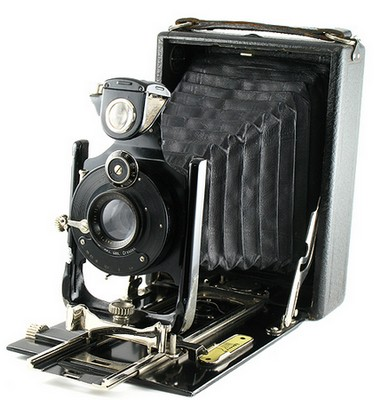
\includegraphics[scale=0.4]{appareil-photo-vintage.jpg}
\end{center}
\begin{block}{}
\begin{center}
Correction du TP : Appareille Photo
\end{center}
\end{block}
\end{frame}

\section{Fragments}

\begin{frame}
\frametitle{Les fragments}

\begin{center}

\includegraphics[scale=0.165]{fragments_glass.jpg}
\end{center}

\begin{block}{}
\begin{center}
\verb!FragmentActivity!
\end{center}
\end{block}
\end{frame}

\begin{frame}
\frametitle{Fragments}
\begin{block}{Qu'est-ce qu'un fragment?}
C'est une partie modulaire d'une activité.
\end{block}

\begin{center}
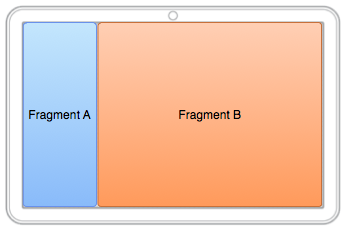
\includegraphics[scale=0.5]{fragments-screen-tab.png}
\end{center}
\end{frame}

\begin{frame}
\frametitle{Fragments}

\begin{block}{Pourquoi utiliser des fragments ?}
Pour permettre a nos applications de s'adapter aux supports physique.
\end{block}

\begin{center}
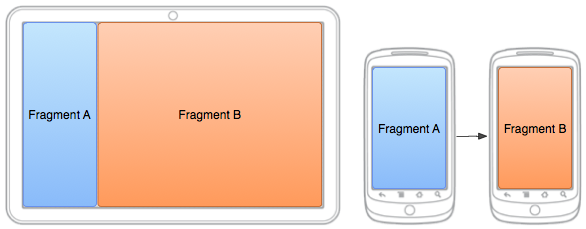
\includegraphics[scale=0.5]{fragments-screen-mock.png}
\end{center}
\end{frame}

\begin{frame}
\frametitle{Créer un fragment}
\begin{block}{Comment faire?}
Comme une Activité.
\end{block}

\begin{block}{Une subtilité :}
C'est la méthode \verb!onCreateView()! que l'on redéfinit, et non \verb!onCreate()!.
\end{block}
\end{frame}


\begin{frame}[fragile]
\frametitle{Un fragment vide}
\begin{block}{Code pour créer un fragment}
\lstset{language=java}
\begin{lstlisting}
import android.os.Bundle;
import android.support.v4.app.Fragment;
import android.view.LayoutInflater;
import android.view.ViewGroup;

public class ArticleFragment extends Fragment {
    @Override
    public View onCreateView(LayoutInflater inflater, ViewGroup container,
        Bundle savedInstanceState) {
        // Inflate the layout for this fragment
        return inflater.inflate(R.layout.article_view, container, false);
    }
}
\end{lstlisting}
\end{block}
\end{frame}

\begin{frame}
\frametitle{Ajouter un fragment à son activité}
\begin{block}{Ajouter un fragment via XML}
On peux ajouter du code XML dans layout-large, et un autre dans layout.
\end{block}
\begin{center}

\includegraphics[scale=0.05]{xml-file.png}
\end{center}
\begin{block}{Ajouter un fragment via l'API}
A l’exécution, on peux déterminer la résolution de l’écran et dynamiquement remodeler l'interface.
\end{block}
\begin{center}

\includegraphics[scale=0.05]{api.png}
\end{center}
\end{frame}

\begin{frame}[fragile]
\frametitle{Ajouter un fragment via XML}
\begin{block}{Code pour ajouter deux fragments}
\lstset{language=xml}
\begin{lstlisting}
<LinearLayout ...>
    <fragment android:name="com.example.android.fragments.HeadlinesFragment"
              android:id="@+id/headlines_fragment"
              android:layout_weight="1"
              android:layout_width="0dp"
              android:layout_height="match_parent" />

    <fragment android:name="com.example.android.fragments.ArticleFragment"
              android:id="@+id/article_fragment"
              android:layout_weight="2"
              android:layout_width="0dp"
              android:layout_height="match_parent" />

</LinearLayout>

\end{lstlisting}
\end{block}
\end{frame}

\begin{frame}[fragile]
\frametitle{Ajouter un fragment à l'exécution}

\begin{block}{\verb!FragmentManager!}
Il nous faut un gestionaire de fragment (\verb!FragmentManager!) pour construire un \verb!FragmentTansaction! qui lui pouras ajouter / supprimer / remplacer des fragments dans notre activité.
\end{block}
\pause
\begin{alertblock}{Il faut un containeur}
Il faut un containeur de type \verb!View! pour y placer nos fragments. Un simple
\lstset{language=xml}
\begin{lstlisting}
<FrameLayout xmlns:android="http://schemas.android.com/apk/res/android"
    android:id="@+id/fragment_container"
    android:layout_width="match_parent"
    android:layout_height="match_parent" />
\end{lstlisting}
    convient.
\end{alertblock}
\end{frame}









\end{document}
